% In this file you should put the actual content of the blueprint.
% It will be used both by the web and the print version.
% It should *not* include the \begin{document}
%
% If you want to split the blueprint content into several files then
% the current file can be a simple sequence of \input. Otherwise It
% can start with a \section or \chapter for instance.

\chapter{Basic theory of magmas}

\begin{definition}[Magma]\label{magma-def}\lean{Magma}\leanok A \emph{magma} is a set $G$ equipped with a binary operation $\circ: G \times G \to G$.  A \emph{homomorphism} $\varphi : G \to H$ between two magmas is a map such that $\varphi(x \circ y) = \varphi(x) \circ \varphi(y)$ for all $x,y \in G$.  An \emph{isomorphism} is an invertible homomorphism.
\end{definition}

Groups, semi-groups, and monoids are familiar examples of magmas.  However, in general we do not expect magmas to have any associative properties.

A magma is called \emph{empty} if it has cardinality zero, \emph{singleton} if it has cardinality one, and \emph{non-trivial} otherwise.

The number of magma structures on a set $G$ of cardinality $n$ is of course $n^{n^2}$, which is \footnote{All sequences start from $n=0$ unless otherwise specified.}
$$ 1, 1, 16, 19683, 4294967296, 298023223876953125, \dots$$
(\href{https://oeis.org/A002489}{OEIS A002489}).
Up to isomorphism, the number of finite magmas of cardinality $n$ up to isomorphism is the slightly slower growing sequence
$$ 1, 1, 10, 3330, 178981952, 2483527537094825, 14325590003318891522275680, \dots$$
(\href{https://oeis.org/A001329}{OEIS A001329}).

\begin{definition}[Free Magma]\label{free-magma-def}\lean{FreeMagma}\leanok\uses{magma-def} The \emph{free magma} $M_X$ generated by a set $X$ (which we call an \emph{alphabet}) is the set of all finite formal expressions built from elements of $X$ and the operation $\circ$.  An element of $M_X$ will be called a \emph{word} with alphabet $X$.  The \emph{order} of a word is the number of $\circ$ symbols needed to generate the word.  Thus for instance $X$ is precisely the set of words of order $0$ in $M_X$.
\end{definition}

For sake of concreteness, we will take the alphabet $X$ to default to the natural numbers $\N$ if not otherwise specified.

For instance, if $X = \{0,1\}$, then $M_X$ would consist of the following words:
\begin{itemize}
  \item $0$, $1$ (the words of order $0$);
  \item $0 \circ 0$, $0 \circ 1$, $1 \circ 0$, $1 \circ 1$ (the words of order $1$);
  \item $0 \circ (0 \circ 0)$, $0 \circ (0 \circ 1)$, $0 \circ (1 \circ 0)$, $0 \circ (1 \circ 1)$, $1 \circ (0 \circ 0)$, $1 \circ (0 \circ 1)$, $1 \circ (1 \circ 0)$, $1 \circ (1 \circ 1)$, $(0 \circ 0) \circ 0$, $(0 \circ 0) \circ 1$, $(0 \circ 1) \circ 0$, $(0 \circ 1) \circ 1$, $(1 \circ 0) \circ 0$, $(1 \circ 0) \circ 1$, $(1 \circ 1) \circ 0$, $(1 \circ 1) \circ 1$ (the words of order $2$);
  \item etc.
\end{itemize}

\begin{lemma} \leanok \lean{FreeMagma.elementsOfNumNodesEq_card_eq_catalan_mul_pow} For a finite alphabet $X$, the number of words of order $n$ is $C_n |X|^{n+1}$, where $C_n$ is the $n^{\mathrm{th}}$ Catalan number and $X$ is the cardinality of $X$.
\end{lemma}

\begin{proof} \leanok Follows from standard properties of Catalan numbers.
\end{proof}

The first few Catalan numbers are
$$ 1, 1, 2, 5, 14, 42, 132, \dots$$
(\href{https://oeis.org/A000108}{OEIS A000108}).


\begin{definition}[Induced homomorphism]\label{induced-def}\uses{free-magma-def}  Given a function $f: X \to G$ from an alphabet $X$ to a magma $G$, the \emph{induced homomorphism} $\varphi_f: M_X \to G$ is the unique extension of $f$ to a magma homomorphism.  Similarly, if $\pi \colon X \to Y$ is a function, we write $\pi_* \colon M_X \to M_Y$ for the unique extension of $\pi$ to a magma homomorphism.
\end{definition}

For instance, if $f : \{0,1\} \to G$ maps $0,1$ to $x,y$ respectively, then
$$ \varphi_f(0 \circ 1) = x \circ y$$
$$ \varphi_f(1 \circ (0 \circ 1)) = y \circ (x \circ y)$$
and so forth.  If $\pi \colon \N \to \N$ is the map $\pi(n) := n+1$, then
$$ \pi_*(0 \circ 1) = 1 \circ 2$$
$$ \pi_*(1 \circ (0 \circ 1)) = 2 \circ (1 \circ 2)$$
and so forth.

\begin{definition}[Law]\label{law-def}\uses{induced-def}\lean{MagmaLaw}  Let $X$ be a set. A \emph{law} with alphabet $X$ is a formal expression of the form $w \formaleq w'$, where $w, w' \in M_X$ are words with alphabet $X$ (thus one can identify laws with alphabet $X$ with elements of $M_X \times M_X$).  A magma $G$ \emph{satisfies}\lean{satisfies} the law $w \formaleq w'$ if we have $\varphi_f( w ) = \varphi_f ( w' )$ for all $f: X \to G$, in which case we write $G \models w \formaleq w'$.
\end{definition}

Thus, for instance, the commutative law
\begin{equation}\label{comm-law}
  0 \circ 1 \formaleq 1 \circ 0
\end{equation}
is satisfied by a magma $G$ if and only if
\begin{equation}\label{comm-law-2}
 x \circ y = y \circ x
\end{equation}
for all $x, y \in G$.  We refer to \eqref{comm-law-2} as the \emph{equation} associated to the law \eqref{comm-law}.  One can think of equations as the ``semantic'' intrepretation of a ``syntactic'' law.  However, we shall often abuse notation and a law with its associated equation thus we shall (somewhat carelessly) also refer to \eqref{comm-law-2} as ``the commutative law'' (rather than ``the commutative equation'').

\begin{lemma}[Pushforward]\label{push}\uses{law-def}  Let $w \formaleq w'$ be a law with some alphabet $X$, $G$ be a magma, and $\pi: X \to Y$ be a function.  If $G \models w \formaleq w'$, then $G \models \pi_*(w) \formaleq \pi_*(w')$.  In particular, if $\pi$ is a bijection, the statements If $G \models w \formaleq w'$, then $G \models \pi_*(w) \formaleq \pi_*(w')$ are equivalent.
\end{lemma}

If $\pi$ is a bijection, we will call $\pi_*(w) \formaleq \pi_*(w')$ a \emph{relabeling} of the law $w \formaleq w'$.  Thus for instance
$$ 5 \circ 7 \formaleq 7 \circ 5$$
is a relabeling of the commutative law \eqref{comm-law}.  By the above lemma, relabeling does not affect whether a given magna satisfies a given law.

\begin{proof}  Trivial.
\end{proof}

\begin{lemma}[Equivalence]\label{equiv}\uses{law-def}  Let $G$ be a magma and $X$ be an alphabet.  Then the relation $G \models w \formaleq w'$ is an equivalence relation on $M_X$.
\end{lemma}

\begin{proof}  Trivial.
\end{proof}

Define the total order of a law $w \formaleq w'$ to be the sum of the orders of $w$ and $w'$.

\begin{lemma}[Counting laws up to relabeling]\label{law-count}\uses{push}  Up to relabeling, the number of laws $w \formaleq w'$ of total order $n$ is $C_{n+1} B_{n+2}$.
\end{lemma}

\begin{proof} Follows from the properties of Catalan and Bell numbers.
\end{proof}

The first few Bell numbers are
$$ 1, 1, 2, 5, 15, 52, 203, \dots$$
(\href{https://oeis.org/A000110}{OEIS A000110}).

The sequence in Lemma \ref{law-count} is
$$ 2, 10, 75, 728, 8526, 115764, \dots$$
(\href{https://oeis.org/A289679}{OEIS A289679}).

Now we would also like to count laws up to relabeling and symmetry.

\begin{lemma}[Counting laws up to relabeling and symmetry]\label{law-count-sym}\uses{push} Up to relabeling and symmetry, the number of laws $w \formaleq w'$ of total order $n$ is
$$ C_{n+1} B_{n+2}/2$$
when $n$ is odd, and
$$ (C_{n+1} B_{n+2} + C_{n/2} (2D_{n+2} - B_{n+2}))/2$$
when $n$ is even, where $D_n$ is the number of partitions of $[n]$ up to reflection.
\end{lemma}

\begin{proof} Elementary counting.
\end{proof}

The sequence $D_n$ is
$$ 1, 1, 2, 4, 11, 32, 117, \dots$$
(\href{https://oeis.org/A103293}{OEIS A103293}), and the sequence in Lemma \ref{law-count-sym} is
$$ 2, 5, 41, 364, 4294, 57882, 888440, \dots$$

We can also identify all laws of the form $w \formaleq w$ with the trivial law $0 \formaleq 0$.  The number of such laws of total order $n$ is zero if $n$ is odd, and $C_{n/2} B_{n/2+1}$ if $n$ is even.  We conclude:

\begin{lemma}[Counting laws up to relabeling, symmetry, and triviality]  Up to relabeling, symmetry, and triviality, the number of laws of total order $n$ is
$$ C_{n+1} B_{n+2}/2$$
if $n$ is odd, $2$ if $n = 0$, and
$$ (C_{n+1} B_{n+2} + C_{n/2} (2D_{n+2} - B_{n+2}))/2 - C_{n/2} B_{n/2+1}$$
if $n \geq 2$ is even.
\end{lemma}

\begin{proof} Routine counting.
\end{proof}

This sequence is
$$2, 5, 39, 364, 4284, 57882, 888365, \dots$$

In particular, up to relabeling, symmetry, and triviality, there are exactly $4694$ laws of total order at most $4$.  A list can be found \href{https://github.com/teorth/equational_theories/blob/main/data/equations.txt}{here}.  A script for generating them may be found \href{https://github.com/teorth/equational_theories/blob/main/scripts/generate_eqs_list.py}{here}.  The list is sorted by the total number of operations, then by the number of operations on the LHS. Within each such class we define an order on expressions by variable $<$ operation, and lexical order on variables.

\chapter{Equations}

\begin{definition}[Equation 1]\label{eq1}\lean{Equation1}\leanok\uses{magma-def}  Equation 1 is the law $x=x$.
\end{definition}

\begin{definition}[Equation 2]\label{eq2}\lean{Equation2}\leanok\uses{magma-def}  Equation 2 is the law $x=y$.
\end{definition}

\begin{definition}[Equation 3]\label{eq3}\lean{Equation3}\leanok\uses{magma-def}  Equation 3 is the law $x=x \circ x$.
\end{definition}

\begin{definition}[Equation 4]\label{eq4}\lean{Equation4}\leanok\uses{magma-def}  Equation 4 is the law $x=x \circ y$.
\end{definition}

\begin{definition}[Equation 5]\label{eq5}\lean{Equation5}\leanok\uses{magma-def}  Equation 5 is the law $x=y \circ x$.
\end{definition}

\begin{definition}[Equation 6]\label{eq6}\lean{Equation6}\leanok\uses{magma-def}  Equation 6 is the law $x=y \circ y$.
\end{definition}

\begin{definition}[Equation 7]\label{eq7}\lean{Equation7}\leanok\uses{magma-def}  Equation 7 is the law $x=y \circ z$.
\end{definition}

\begin{definition}[Equation 8]\label{eq8}\lean{Equation8}\leanok\uses{magma-def}  Equation 8 is the law $x=x \circ (x \circ x)$.
\end{definition}

\begin{definition}[Equation 42]\label{eq42}\lean{Equation42}\leanok\uses{magma-def}  Equation 42 is the law $x \circ y = x \circ z$.
\end{definition}

\begin{definition}[Equation 43]\label{eq43}\lean{Equation43}\leanok\uses{magma-def}  Equation 43 is the law $x \circ y = y \circ x$.
\end{definition}

\begin{definition}[Equation 46]\label{eq46}\lean{Equation46}\leanok\uses{magma-def}  Equation 46 is the law $x \circ y = z \circ w$.
\end{definition}

\begin{definition}[Equation 168]\label{eq168}\lean{Equation168}\leanok\uses{magma-def}  Equation 168 is the law $x = (y \circ x) \circ (x \circ z)$.
\end{definition}

\begin{definition}[Equation 387]\label{eq387}\lean{Equation387}\leanok\uses{magma-def}  Equation 387 is the law $x \circ y = (y \circ y) \circ x$.
\end{definition}

\begin{definition}[Equation 4512]\label{eq4512}\lean{Equation4512}\leanok\uses{magma-def}  Equation 4512 is the law $x \circ (y \circ z) = (x \circ y) \circ z$.
\end{definition}

\begin{definition}[Equation 4513]\label{eq4513}\lean{Equation4513}\leanok\uses{magma-def}  Equation 4513 is the law $x \circ (y \circ z) = (x \circ y) \circ w$.
\end{definition}

\begin{definition}[Equation 4552]\label{eq4552}\lean{Equation4552}\leanok\uses{magma-def}  Equation 4552 is the law $x \circ (y \circ z) = (x \circ w) \circ u$.
\end{definition}

\begin{definition}[Equation 4582]\label{eq4582}\lean{Equation4582}\leanok\uses{magma-def}  Equation 4582 is the law $x \circ (y \circ z) = (w \circ u) \circ v$.
\end{definition}

\chapter{General implications}

We will be interested in seeing which laws imply which other laws, in the sense that magmas obeying the former law automatically obey the latter.  We will also be interested in \emph{anti-implications} showing that one law does \emph{not} imply another, by producing examples of magmas that obey the former law but not the latter. Here is a formal definition.

\begin{definition}[Implication]\label{impl}\uses{law-def}  A law $w  \formaleq  w'$ is said to \emph{imply} another law $w''  \formaleq  w'''$, if every magma $G$ that satisfies the former, satisfies the latter:
  $$ G \models w  \formaleq  w' \implies G \models w''  \formaleq  w'''.$$
Two laws are said to be \emph{equivalent} if they imply each other.
\end{definition}

\begin{lemma}[Pre-order]\label{pre-order}\uses{impl}  Implication is a pre-order on the set of laws, and equivalence is an equivalence relation.
\end{lemma}

\begin{proof} Trivial.
\end{proof}

Implications between the laws from Chapter \ref{subgraph-eq} are depicted in Figure \ref{fig:implications}.

\begin{figure}
  \centering
  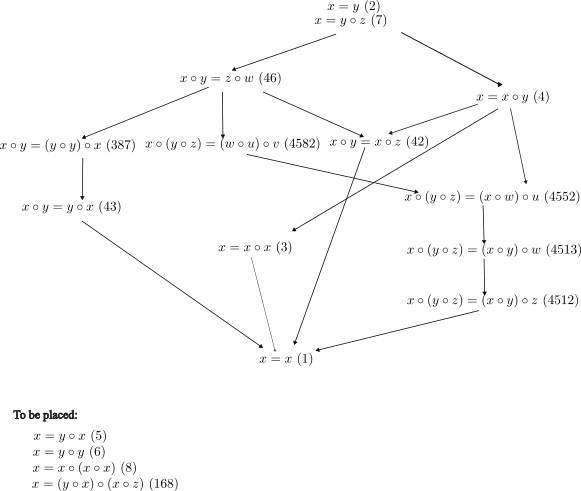
\includegraphics[width=0.5\linewidth]{../../images/implications.png}
  \caption{Implications between the above equations, displayed as a Hasse diagram.}
  \label{fig:implications}
\end{figure}


\begin{lemma}[Minimal element]\label{minimal}\uses{pre-order}  The law $0  \formaleq  0$ is the minimal element in this pre-order.
\end{lemma}

\begin{proof} Trivial.
\end{proof}

\begin{lemma}[Maximal element]\label{maximal}\uses{pre-order}  The law $0  \formaleq  0$ is the minimal element in this pre-order.
\end{lemma}

\begin{proof} Trivial.
\end{proof}

Every magma $G$ has a \emph{reversal} $G^{\mathrm{op}}$, formed by by replacing the magma operation $\circ$ with its opposite $\circ^{\mathrm{op}}:(x,y) \mapsto y \circ x$. There is a natural isomorphism between these magmas, which induces an involution $w \mapsto w^{\mathrm{op}}$ on words $w \in M_X$.  Every law $w  \formaleq  w'$ then has a \emph{dual} $w^{\mathrm{op}}  \formaleq  (w')^{\mathrm{op}}$.

For instance, the dual of the law $0 \circ 1 = 0 \circ 2$ is $1 \circ 0 = 2 \circ 0$, which after relabeling is $0 \circ 1 = 2 \circ 1$.  A list of equations and their duals can be found \href{https://github.com/teorth/equational_theories/blob/main/data/dual_equations.md}{here}.  Of the 4694 equations under consideration, 84 are self-dual, leaving 2305 pairs of dual equations.

The pre-ordering on laws has a duality symmetry:

\begin{lemma}[Duality of laws]\label{duality}\uses{pre-order}  If $w  \formaleq  w'$ implies $w''  \formaleq  w'''$, then $w^{\mathrm{op}}  \formaleq  (w')^{\mathrm{op}}$ implies $w''^{\mathrm{op}}  \formaleq  (w''')^{\mathrm{op}}$.
\end{lemma}

\begin{proof} This follows from the fact that a magma $G$ satisfies a law $w  \formaleq  w'$ if and only if $G^{\mathrm{op}}$ satisfies $w^{\mathrm{op}}  \formaleq  (w')^{\mathrm{op}}$.
\end{proof}

Some equational laws can be ``diagonalized'':

\begin{theorem}[Diagonalization]\label{diag}  An equational law of the form
  \begin{equation}\label{prediag} F(x_1,\dots,x_n) = G(y_1,\dots,y_m),
  \end{equation}
  where $x_1,\dots,x_n$ and $y_1,\dots,y_m$ are distinct elements of the alphabet, implies the diagonalized law
$$ F(x_1,\dots,x_n) = F(x'_1,\dots,x'_n).$$
where $x'_1,\dots,x'_n$ are distinct from $x_1,\dots,x_n$
In particular, if $G(y_1,\dots,y_m)$ can be viewed as a specialization of $F(x'_1,\dots,x'_n)$, then these two laws are equivalent.
\end{theorem}

\begin{proof}  From two applications of \eqref{prediag} one has
$$ F(x_1,\dots,x_n) = G(y_1,\dots,y_m)$$
and
$$ F(x'_1,\dots,x'_n) = G(y_1,\dots,y_m)$$
whence the claim.
\end{proof}

Thus for instance, Definition \ref{eq7} is equivalent to Definition \ref{eq2}.

\begin{theorem}[Laws implied by the constant law]\label{constant-impl}\uses{impl,eq46}  If $w, w'$ each have order at least one, then the law $w \formaleq w'$ is implied by the constant law (Definition \ref{eq46}).  If exactly one of $w, w'$ has order zero, and the law $w \formaleq w'$ is not implied by the constant law.
\end{theorem}

\begin{proof} Routine.
\end{proof}

\begin{theorem}[Criterion for implication]\label{variable-impl}\uses{impl}  If $w \formaleq w'$ is such that every variable appears the same number of times in both $w$ and $w'$, and $w \formaleq w'$ implies another law $w'' \formaleq w'''$, then every variable appears the same number of times in both $w''$ and $w'''$.
\end{theorem}

\begin{proof} Consider the magma $\R$ with the addition law $+$.  By hypothesis, this magma obeys $w \formaleq w'$, and hence $w'' \formaleq w'''$, giving the claim by comparing coefficients of the linear forms associated to $w''$ and $w'''$ in this magma.
\end{proof}

\chapter{Completeness and compactness theorems}

We now generalize the implication concept from Definition \ref{impl}:

\begin{definition}[Semantic consequence]\label{semantic-def}\uses{law-def} Let $\Gamma$ be a collection of laws, and let $E$ be a law. We say that $E$ is a \emph{semantic consequence} of $\Gamma$, and write $\Gamma \models E$, if every magma that obeys every law in $\Gamma$, also obeys $E$.
\end{definition}

Definition \ref{impl} is basically the case where $\Gamma$ is a singleton.

\begin{definition}[Syntactic consequence]\label{syntactic-def}\uses{law-def, push} Let $\Gamma$ be a collection of laws, and let $E$ be a law. We say that $E$ is a \emph{syntactic consequence} of $\Gamma$, and write $\Gamma \vdash E$, if $E$ can be deduced from $\Gamma$ using the following rules of inference:
\begin{itemize}
\item If $E$ is an element of $\Gamma$, then $\Gamma \vdash E$.
\item For any word $w$, we have $\Gamma \vdash w \formaleq w$.
\item If $w,w'$ are words with $\Gamma \vdash w \formaleq w'$, then $\Gamma \vdash w' \formaleq w$.
\item If $w,w',w''$ are words with $\Gamma \vdash w \formaleq w'$ and $\Gamma \vdash w' \formaleq w''$, then $\Gamma \vdash w \formaleq w''$.
\item If $w,w'$ are words with $\Gamma \vdash w \formaleq w'$, and $\pi : \N \to \N$ is a function, then $\Gamma \vdash \pi_* w \formaleq \pi_* w'$.
\item If $w,w',v$ are words with $\Gamma \vdash w \formaleq w'$, then $\Gamma \vdash v \circ w \formaleq v \circ w'$ and $\Gamma \vdash w \circ v \formaleq w' \circ v$.
\end{itemize}
\end{definition}

\begin{theorem}[Completeness theorem]\label{completeness-thm}\uses{semantic-def,syntactic-def}  Let $\Gamma$ be a collection of laws, and let $E$ be a law.  Then $\Gamma \models E$ if and only if $\Gamma \vdash E$.
\end{theorem}

\begin{proof} (Sketch) The `only if' component is soundness, and follows from verifying that the rules of inference in Definition \ref{syntactic-def} holds for $\models$.  The `if` part is completeness, and is proven by constructing the magma of words, quotiented out by the relation $\Gamma \vdash w \formaleq w'$, which is easily seen to be an equivalence relation respecting the magma operation
\end{proof}

\begin{corollary}[Compactness theorem]\label{compactness-thm}\uses{semantic-def,syntactic-def}  Let $\Gamma$ be a collection of laws, and let $E$ be a law.  Then $\Gamma \models E$ if and only if there exists a finite subset $\Gamma'$ of $\Gamma$ such that $\Gamma' \models E$.
\end{corollary}

\begin{proof}\uses{completeness-thm} The claim is obvious for $\vdash$, and the claim then follows from Theorem \ref{completeness-thm}
\end{proof}

\chapter{Implications between selected laws}

We collect here some notable implications between the the selected laws in Chapter \ref{subgraph-eq}.   By Theorem \ref{sound-complete}, every implication can basically be established by a finite number of rewrites.  In most cases, the sequence of rewrites is quite straightforward, and the implication is very easy, but we record some less obvious examples.

\begin{theorem}[387 implies 43]\label{387_implies_43}\uses{eq387,eq43}\lean{Subgraph.Equation387_implies_Equation43}\leanok  Definition \ref{eq387} implies Definition \ref{eq43}.
\end{theorem}

\begin{proof}\leanok (From \href{https://mathoverflow.net/a/450905/766}{MathOverflow}).
  By Definition \ref{eq387}, one has the law
\begin{equation}\label{387-again}
  (x \op x) \op y = y \op x.
\end{equation}
Specializing to $y=x \op x$, we conclude
$$(x \op x) \op (x \op x) = (x \op x) \op x$$
and hence by another application of \eqref{eq387} we see that $x \op x$ is idempotent:
\begin{equation}\label{idem}
  (x \op x) \op (x \op x) = x \op x.
\end{equation}
Now, replacing $x$ by $x \op x$ in \eqref{387-again} and then using \eqref{idem} we see that
$$ (x \op x) \op y = y \op (x \op x)$$
so in particular $x \op x$ commutes with $y \op y$:
\begin{equation}\label{op-idem} (x \op x) \op (y \op y) = (y \op y) \op (x \op x).
\end{equation}
Also, from two applications of \eqref{387-again} one has
$$(x \op x) \op (y \op y) = (y \op y) \op x = x \op y.$$
Thus \eqref{op-idem} simplifies to $x \op y = y \op x$, which is Definition \ref{eq43}.
\end{proof}

\begin{theorem}[29 equivalent to 14]\label{29_equiv_14} \uses{eq29,eq14}\lean{Subgraph.Equation29_implies_Equation14}\leanok  Definition \ref{eq29} is equivalent to Definition \ref{eq14}.
\end{theorem}

This result was posed as Problem A1 from Putnam 2001.

\begin{proof}\leanok\uses{duality} By Lemma \ref{duality} it suffices to show that Definition \ref{eq29} implies Definition \ref{eq14}.  From Definition \ref{eq29} one has
  $$ x = ((x \op y) \op x) \op (x \op y)$$
  and also
  $$ y = (x \op y) \op x$$
  giving $x = y \op (x \op y)$, which is Definition \ref{eq14}.
\end{proof}

\begin{theorem}[14 implies 29]\label{14_implies_29} \uses{eq29,eq14}\lean{Subgraph.Equation14_implies_Equation29}\leanok  Definition \ref{eq14} implies Definition \ref{eq29}.
\end{theorem}

This result was posed as Problem A1 from Putnam 2001.

\begin{proof}\leanok
\end{proof}

The following result was Problem A4 on Putnam 1978.

\begin{theorem}[3744 implies 3722, 381]\label{3744_implies_3722_381}\uses{eq3744, eq3722, eq381}\lean{Subgraph.Equation3744_implies_Equation3722, Subgraph.Equation3744_implies_Equation381}\leanok Definition \ref{eq3744} implies Definition \ref{eq3722} and Definition \ref{eq381}.
\end{theorem}

\begin{proof}\leanok By hypothesis, one has
$$x \op y = (x \op z) \op (w \op y)
  $$
for all $x,y,z,w$.  Various specializations of this give
\begin{align}
 x \op y &= (x \op z) \op (y \op y) \label{381-1} \\
 x \op z &= (x \op z) \op (x \op z) \label{381-2} \\
(x \op z) \op y &= ((x \op z) \op (x \op z)) \op (y \op y) \label{381-3}.
\end{align}
The equation \eqref{381-2} gives Definition \ref{eq3722}, while \eqref{381-1}, \eqref{381-2}, \eqref{381-3} gives
$$ x \op y = (x\op z) \op y$$
which is Definition \ref{eq381}.
\end{proof}

\begin{theorem}[1689 is equivalent to 2]\label{1689_equiv_2}\uses{eq1689, eq2}\lean{Subgraph.Equation1689_implies_Equation2, Subgraph.Equation2_implies_Equation1689}\leanok Definition \ref{eq1689} is equivalent to Definition \ref{eq2}.
\end{theorem}


\begin{proof}\leanok  The implication of Definition \ref{eq1689} from Definition \ref{eq2} is trivial.  The converse is a surprisingly long chain of implications; see pages 326--327 of \cite{Kisielewicz2}.  The initial law
$$ x = (y \op x) \op ((x \op z) \op z)$$
is used to obtain, in turn,
$$ x \op ((((x \op y) \op y) \op z) \op z) = (x \op y) \op y,$$
$$(x \op (y \op z)) \op (z \op ((z \op w) \op w)) = y \op z,$$
$$x \op (y \op ((y \op z) \op z)) = (x \op y) \op y,$$
$$((x \op (y \op z)) \op z) \op z = y \op z,$$
$$(x \op (y \op (z \op w))) \op (z \op w) = y \op (z \op w),$$
$$(x \op (y \op z)) \op (y \op z) = x \op (y \op z),$$
$$((x \op y) \op ((y \op z) \op z)) \op ((y \op z) \op z) = y,$$
$$((x \op y) \op ((y \op z) \op z)) \op ((y \op z) \op z) = ((x \op ((x \op y) \op ((y \op z) \op z))) \op ((y \op z) \op z)) \op ((y \op z) \op z),$$
$$ x \op ((x \op y) \op y) = x,$$
$$ x \op (x \op (y \op z)) = x,$$
$$ (x \op y) \op y = x \op y,$$
$$ (x \op x) \op x = x,$$
$$ (x \op y) \op y = y,$$
$$ x \op y = y.$$
\end{proof}

The following result was established in \cite{mendelsohn-padmanabhan}.

\begin{theorem}[Consequences of 1571]\label{1571_impl}\uses{eq1571, eq2662, eq40, eq23, eq8, eq16, eq14, eq43, eq4512}\lean{Subgraph.Equation1571_implies_Equation2662, Subgraph.Equation1571_implies_Equation40, Subgraph.Equation1571_implies_Equation23,Subgraph.Equation1571_implies_Equation8, Subgraph.Equation1571_implies_Equation16, Subgraph.Equation1571_implies_Equation43, Subgraph.Equation1571_implies_Equation4512}\leanok  Magmas obeying Definition \ref{eq1571} also obey Definitions \ref{eq2662}, \ref{eq40}, \ref{eq23}, \ref{eq8}, \ref{eq16}, \eqref{eq14}, \ref{eq43}, and \ref{eq4512}, and are in fact abelian groups of exponent two.  Conversely, all abelian groups of exponent two obey Definition \ref{eq1571}.
\end{theorem}

\begin{proof}\leanok  Suppose that a magma $G$ obeys Definition \ref{eq1571}, thus
\begin{equation}\label{1571-again}
 x = (y \op z) \op (y \op (x \op z)).
\end{equation}
$$ x = ((x \op y) \op (x \op y)) \op ((x \op y) \op (x \op (x \op y)))$$
and
$$ x = (x \op y) \op (x \op (x \op y))$$
whence
$$x = ((x \op y) \op (x \op y)) \op x$$
which is Definition \ref{eq2662}.  This gives
$$y = ((y \op z) \op (y \op z)) \op y$$
while from \eqref{1571-again} one has
$$ (y \op z) \op (y \op z) = (x \op y) \op (x \op ((y \op z) \op (y \op z) \op y))$$
whence
$$ (x \op y) \op (x \op y) = (y \op z) \op (y \op z).$$
This implies that $(x \op y) \op (x \op y)$ does not depend on $x$, or on $y$, hence is equal to some constant $e$:
$$ (x \op y) \op (x \op y) = e.$$
From \eqref{1571-again} the magma operation is surjective, hence
\begin{equation}\label{xxe} x \op x = e
\end{equation}
which gives Definition \ref{eq40}.  Applying \eqref{1571-again} with $x=y=z$ we conclude
$$ x = e \op (x \op e)$$
while if we instead take $y=z=e$ we have
$$ x = e \op (e \op (x \op e))$$
hence
$$ x = e \op x$$
and then also
$$ x = x \op e$$
from which we readily conclude Definitions \ref{eq23}, \ref{eq8}; thus $e$ is an identity element.  From \eqref{1571-again} with $z=e$ we now have
\begin{equation}\label{16-again}
 x = y \op (y \op x)
\end{equation}
which is Definition \ref{eq16}. If instead we take $y=e$ we have
\begin{equation}\label{14-again}
  x = z \op (x \op z)
\end{equation}
which is Definition \ref{eq14}.  So if we substitute $z = x \op y$ and use \eqref{16-again} we obtain
$$ x = (x \op y) \op y$$
and hence
$$ y \op x = y \op ((x \op y) \op y) = x \op y$$
thanks to \eqref{14-again}.  This gives Definition \ref{eq43}, thus $G$ is now commutative.  From \eqref{1571-again} once more one has
$$x \op (y \op z) = (y \op x) \op (z \op ((x \op (y \op z)) \op x))$$
which one can simplify using commutativity and \eqref{16-again} (or \eqref{14-again}) to eventually obtain
$$x \op (y \op z) = (x \op y) \op z$$
which is Definition \ref{eq4512}.  $G$ is now commutative and associative, and every element is its own inverse and of exponent $2$, hence is an abelian group thanks to \eqref{xxe}, so $G$ is an abelian group of exponent $2$ as claimed.  The converse is easily verified.
\end{proof}

\begin{theorem}[953 is equivalent to 2]\label{953_equiv_2}\uses{eq953, eq2}\lean{Subgraph.Equation953_implies_Equation2}\leanok  Definition \ref{eq953} is equivalent to Definition \ref{eq2}.
\end{theorem}

\begin{proof}\leanok  It suffices to show that Definition \ref{eq953} implies Definition \ref{eq2}.  Pick an element $0$ of $G$ and define $1 = 0 \op 0$ and $2 = 1 \op 1$ (we do not require $0,1,2$ to be distinct).
From Definition \ref{eq953} with $x=z=0$ we have
$$ 0 = y \op 2.$$
If we then apply Definition \ref{eq953} with $z=1$ we conclude that
$$ x = y \op 0$$
for all $x,y$, from which one concludes $x=x'$ for any $x,x' \in G$, giving Definition \ref{eq2}.
\end{proof}


Some other notable equational laws are as follows.

\begin{theorem}[Sheffer stroke axiom]\label{sheffer}  The law
$$ 0 \formaleq (1 \op ((0 \op 1) \op 1)) \op (0 \op (2 \op 1))$$
or in equation form
$$ x = y \op ((x \op y) \op y) \op (x \op (z \op y)) $$
axiomatizes the Sheffer stroke operation. {\bf TODO: locate the equation number for this law.}
\end{theorem}

\begin{proof}
See \cite{mccune_et_al}.  In fact this is the shortest law with this property.
\end{proof}

A \emph{natural central groupoid} is, up to isomorphism, a magma with carrier $S \times S$ for some set $S$ and operation
$$ (a,b) \op (c,d) = (b,c).$$
These are examples of central groupoids (Definition \ref{eq168}).

\begin{theorem}[Natural central groupoid axiom]\label{natural-central-groupoid}  The law
$$ 0 \formaleq (1 \op ((2 \op 0) \op 3)) \op (0 \op 3)$$
or in equation form
\begin{equation}\label{26302}
  x = (y \op ((z \op x) \op w)) \op (x \op w)
\end{equation}
(Equation 26302) characterizes natural central groupoids.
\end{theorem}

\begin{proof}
  See \cite[Theorem 5]{knuth}.  The proof is quite lengthy; a sketch is as follows. It is easy to see that natural central groupoids obey \eqref{26302}.  Conversely, if this law holds, then
\begin{align*}
  (y \op z) \op (z \op w) &= (( x \op ((w \op (y \op z)) \op w)) \op ((y \op z) \op w)) \op (z \op w)\\
  &= z
\end{align*}
so we have a central groupoid.  Setting $y = (t \op t) \op t$, $z = t \op (t \op t)$, $w = t \op t$ in \eqref{26302} we also obtain
$$ (x \op t) \op t = (t \op t) \op t.$$
Using the notation
$$ x^{(1)} := (x \op x) \op x, \quad x^{(2)} := x \op (x \op x)$$
we then have
\begin{align*}
  x \op t &= ((x \op x) \op (x \op t)) \op ((x \op t) \op t) \\
  &= x \op t^{(1)}.
\end{align*}
A lengthy computer-assisted argument then gave the dual identity
$$ t^{(2)} \op x = t \op x$$
Together, these give
$$ x^{(2)} \op y^{(1)} = x \op y.$$
Multiplying on the left by $x = x^{(1)}\op x^{(2)}$, one can conclude that
$$ x^{(2)} = x \op (x \op y).$$
One then has
\begin{align*}
  (x \op y)^{(1)} &= ((y \op x) \op (x \op y)) \op (x \op y) \\
&= x \op (x \op y) \\
&= x^{(2)}
\end{align*}
and a similar argument gives
$$ (x \op y)^{(2)} = y^{(1)}.$$
Since $(x \op x)^{(1)} = x^{(2)}$ and $(x \op x)^{(2)} = x^{(1)}$, we conclude that $x^{(1)}$ and $x^{(2)}$ are idempotent.  Since $x = x^{(1)} \op x^{(2)}$, we see that every $x$ is the product of two idempotents.  One can show that this representation is unique, and gives a canonical identification with a natural central groupoid.
\end{proof}

\chapter{Selected magmas}

Each magma can be used to establish anti-implications: if $\Gamma$ is the set of all laws obeyed by a magma $G$, then we have $\not E \leq E'$ whenever $E \in \Gamma$ and $E' \not \in \Gamma$.  Large numbers of implications can already be obtained from

\begin{itemize}
  \item All magmas of order at most $4$, up to isomorphism (of which there are $178,985,294$);
  \item All commutative magmas of order $5$, up to isomorphism {\bf determine their count};
  \item Cyclic groups $\Z/N\Z$ with $2 \leq N \leq 12$ and $x \circ y = ax^2+bxy+cy^2+dx+ey$ for randomly chosen $a,b,c,d,e$.
  \item There are only $1410$ distinct cancellative magmas of order $5$ (up to isomorphism), and Mace4 can generate all of them in under 20 seconds. A shell script to do this is available \href{https://github.com/zaklogician/equational_theories/tree/cancellative_magmas/scripts/cancellative_magmas}{here}. A magma is cancellative if $xy=xz$ implies $y=z$ and $yx=zx$ implies $y=z$.
\end{itemize}


Some other magmas have been used to establish counterexamples:
\begin{itemize}
  \item The cyclic group $\Z/6\Z$ with the addition law.
  \item The natural numbers with law $x \circ y = x+1$.
  \item The natural numbers with law $x \circ y = xy+1$.
  \item The reals with $x \circ y = (x+y)/2$.
  \item The natural numbers with $x \circ x$ equal to $x$ when $x=y$ and $x+1$ otherwise.
\end{itemize}

\chapter{Equivalence with the constant and singleton laws}

\href{https://github.com/teorth/equational_theories/blob/main/equational_theories/Generated/Constant.lean}{85 laws}
have been shown to be equivalent to the constant law (Definition \ref{eq46}), and
\href{https://github.com/teorth/equational_theories/blob/main/equational_theories/Generated/Singleton.lean}{815 laws}
have been shown to be equivalent to the singleton law (Definition \ref{eq2}).

These are the laws up to 4 operations that follow from diagonalization of \ref{eq2} and \ref{eq46}.

To formalize these in Lean, a search was run on the list of equations to discover
diagonalizations of these two specific laws: equations of the form $x = R$ where $R$ doesn't include
$x$, and equations of the form $x \circ y = R$ where $R$ doesn't include $x$ or $y$.

The proofs themselves all look alike, and correspond exactly to the two steps described in the proof
of \ref{diag}. The Lean proofs were generated semi-manually, using search-and-replace starting from
the output of \texttt{grep} that found the diagonalized laws.

In the case of the constant law, equation \ref{eq41} ($x \circ x = y \circ z$) wasn't detected using
this method. It was added manually to the file with the existing proof from the sub-graph project.

\chapter{Simple rewrites}

\href{https://github.com/teorth/equational_theories/tree/main/equational_theories/SimpleRewrites/theorems}{53,905 implications} were automatically generated by simple rewrites.

{\bf describe the process of automatically generating these implications here.}

\chapter{Trivial auto-generated theorems}

\href{https://github.com/teorth/equational_theories/tree/main/equational_theories/Generated/TrivialBruteforce}{Approximately 4.5m transitive implications were proven by a transitive reduction of about 15k theorems}. Most of these implications were derived from being the first automated run to connect the largest equivalence classes, hence creating a large set of transitively closed implications.

Scripts generated theorems to try simple combinations of equation rewrites to reach the desired goal for every unknown implication. The generated proof scripts were run with lean and the successful theorems were extracted. An example of the types of generated rewrites that were tested:

\begin{verbatim}
  repeat intro
  apply
\end{verbatim}

\begin{verbatim}
  repeat intro
  try { rw [<-h] }
  try { rw [<-h, <-h] }
  try { rw [<-h, <-h, <-h] }
  try { rw [<-h, <-h, <-h, <-h] }
  try { rw [<-h, <-h, <-h, <-h, <-h] }
  repeat rw [h]
\end{verbatim}

\begin{verbatim}
  repeat intro
  try {
    nth_rewrite 1 [h]
    try { rw [h] }
    try { rw [<-h] }
  }
  try {
    nth_rewrite 2 [h]
    try { rw [h] }
    try { rw [<-h] }
  }
  try {
    nth_rewrite 3 [h]
    try { rw [h] }
    try { rw [<-h] }
  }
  try {
    nth_rewrite 4 [h]
    try { rw [h] }
    try { rw [<-h] }
  }
  try {
    nth_rewrite 1 [h]
    nth_rewrite 1 [h]
    try { rw [h] }
    try { rw [<-h] }
  }
  ...
\end{verbatim}

\chapter{Enumerating Small Finite Magmas}\label{all-small-magmas-chapter}

{\bf describe the process of automatically generating these implications here.}


\bibliographystyle{plain} % We choose the "plain" reference style
\bibliography{references}
